\documentclass[12pt]{beamer}

%\usepackage[left=2.5cm, right=2.5cm]{geometry}
\usepackage[utf8]{inputenc}
\usepackage[T1]{fontenc}
\usepackage[ngerman]{babel}
\usepackage{colortbl}
%\usepackage[onehalfspacing]{setspace}
\usepackage{amsmath}
\usepackage{amssymb}
\usepackage{csquotes}
\usepackage{hyperref}
\usepackage{algorithm}
\usepackage{algpseudocode}
\usepackage{graphicx}
\usepackage{wrapfig}
\usepackage{tikz}
\usepackage{circuitikz}
\usepackage{tikz-timing}
\usepackage{bytefield}
\usepackage{pgf-umlcd}
\usepackage[backend=biber, style=ieee, citestyle=ieee]{biblatex}
\usepackage{rotating}

\usetheme{Madrid}
\usecolortheme{whale}

\newcounter{listnum}

\title{Mikrocontroller Touchscreen GUI}
\author{Neo Hornberger, Tim Ludwig}
\date{21.01.2022}

\bibliography{../Bibliography.bib}

\begin{document}
	\maketitle	
	\frame{\tableofcontents}
	
	\section{Touchscreen Hardware}
	\begin{frame}{Resistive Touchscreens}
		\begin{columns}
			\begin{column}{0.4\textwidth}
				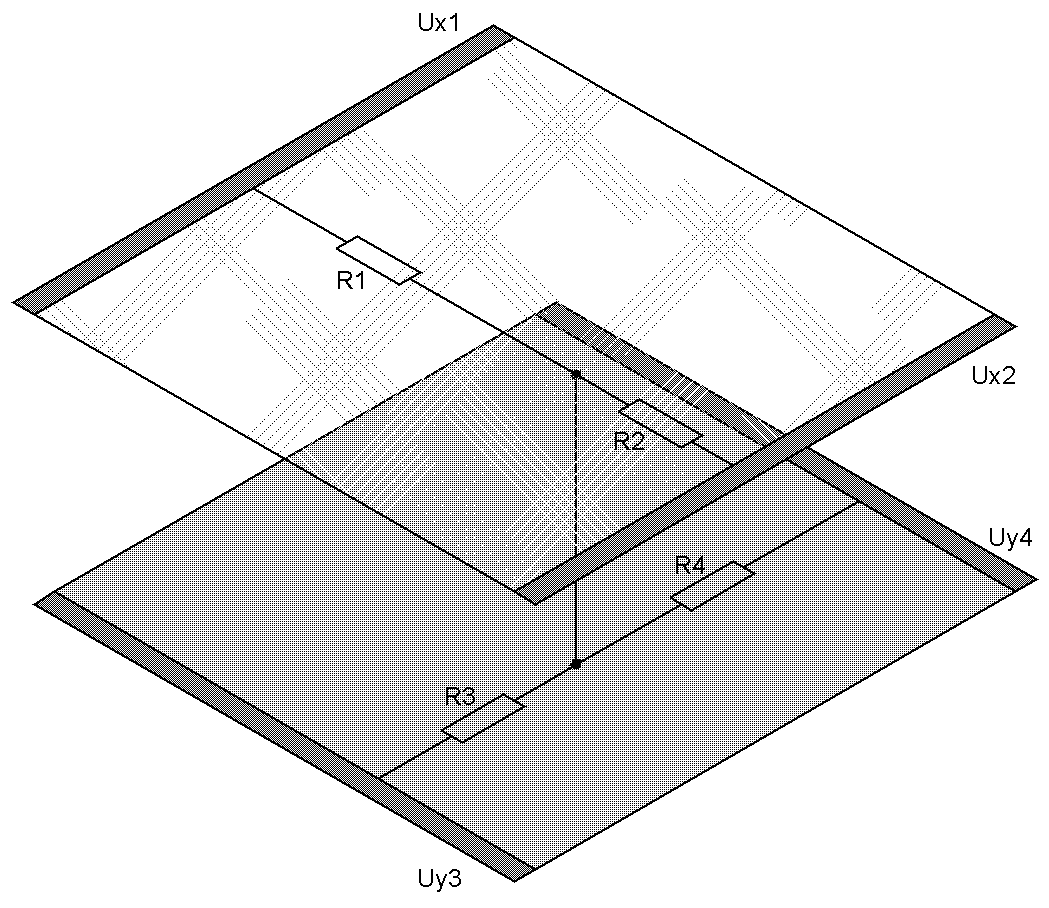
\includegraphics[width=\textwidth]{../Images/ResistiveTouchScreen.png}
			\end{column}
			\begin{column}{0.6\textwidth}
				Funktionsweise: 
				\begin{itemize}
					\item<1-> Kontakt zweier Schichten durch Deformierung
					\item<2-> Anlegen einer Spannung über eine Schicht
					\item<3-> Messen des Potentials an den Enden der anderen Schicht
					\item<4-> Wdh. mit vertauschten Rollen
				\end{itemize}
				
				Häufige Nutzung:
				\begin{itemize}
					\item Kiosksysteme
					\item Industrie
					\item \dots
				\end{itemize}
			\end{column}
		\end{columns}
	\end{frame}

	\begin{frame}{kapazitive Touchscreens}
		Arten von kapazitiven Touchscreens:
		\begin{itemize}
			\item Oberflächen-kapazitiv
			\item Projiziert-kapazitiv
		\end{itemize}
		\medskip
		Häufige Nutzung:
		\begin{itemize}
			\item Smartphones
			\item Tablets
			\item \dots
		\end{itemize}
	\end{frame}

	\begin{frame}{Oberflächen-kapazitive Touchscreens}
		\begin{columns}
			\begin{column}{0.4\textwidth}
				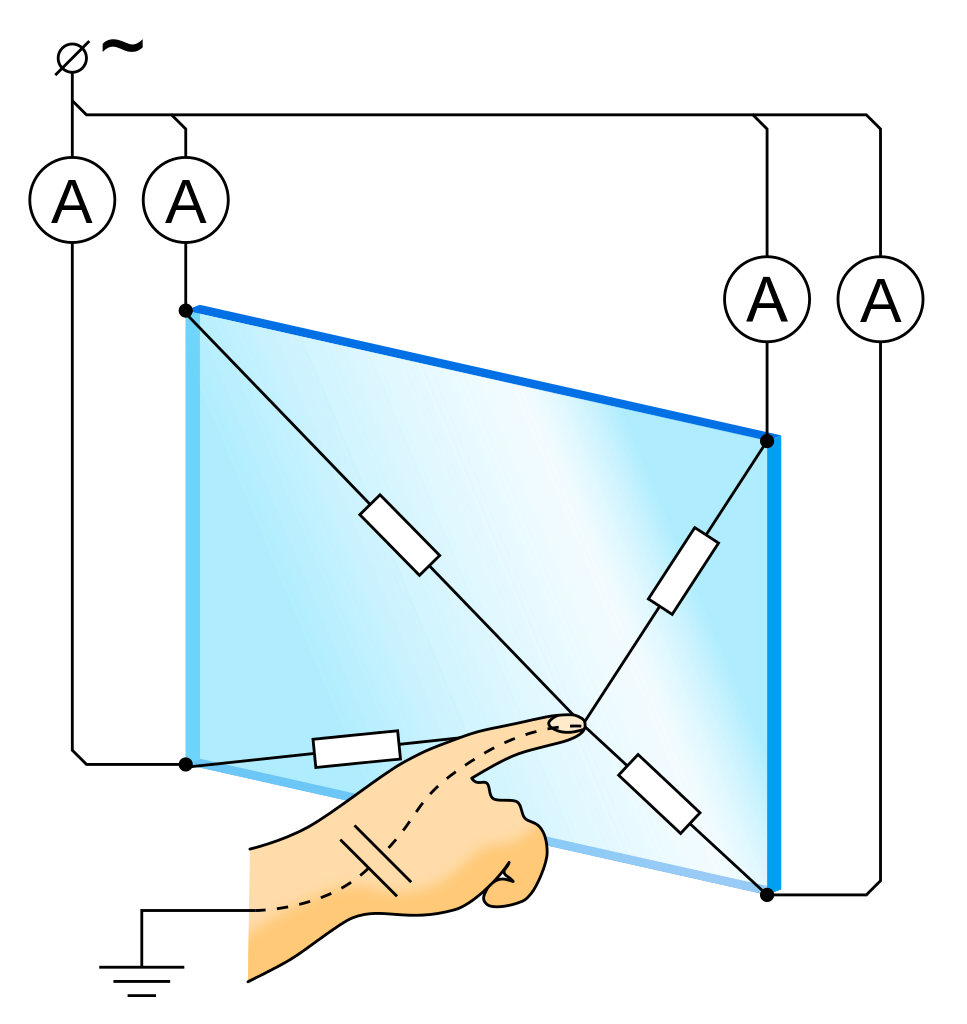
\includegraphics[width=\textwidth]{../Images/SurfaceCapacitiveTouchScreen.png}
				
			\end{column}
			\begin{column}{0.6\textwidth}
				Funktionsweise:
				\begin{itemize}
					\item<1-> Wechselspannung an den Ecken anlegen
					\item<2-> bei Berührung wird eine Kapazität auf- und entladen
					\item<3-> den Strom durch die Ecken messen
				\end{itemize}
			\end{column}
		\end{columns}
	\end{frame}
	
	\begin{frame}{Projiziert-kapazitive Touchscreens}
		\begin{columns}
			\begin{column}{0.4\textwidth}
				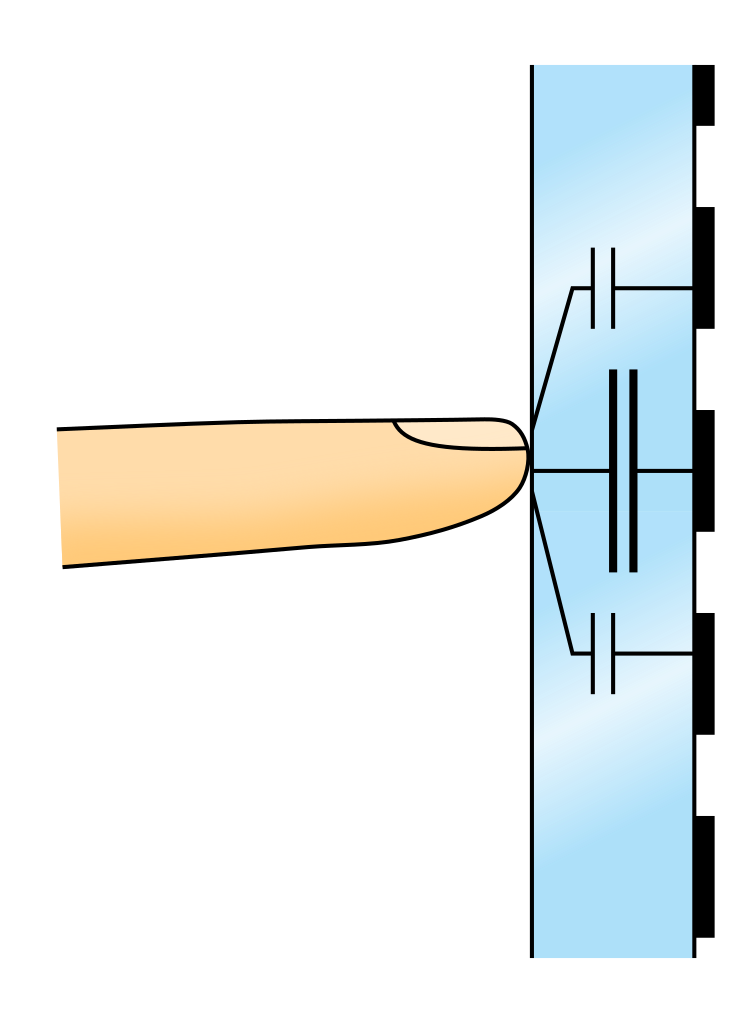
\includegraphics[width=\textwidth]{../Images/ProjectedCapacitiveTouchScreen.png}
			\end{column}
			\begin{column}{0.6\textwidth}
				Funktionsweise:
				\begin{itemize}
					\item<1-> zwei Ebenen Gitter aus Leitern
					\item<2-> Anlegen einer Wechselspannung an eine Ebene
					\item<3-> Messen des durch die Leiter der anderen Ebene fließenden Stroms
				\end{itemize}
			\end{column}
		\end{columns}
	\end{frame}
	
	\begin{frame}{Kapazitiv vs. Resistiv}
		\begin{tabular}{| >{\columncolor{structure.fg!80}\color{white}} l | p{4.5cm} | p{4.5cm} |}
			\hline
			\rowcolor{structure.fg!80} & \color{white}Vorteile & \color{white}Nachteile\\\hline
			kapazitiv & \normalcolor
				\begin{itemize}
					\item geringer Verschleiß
					\item Multitouch
				\end{itemize} &
				\begin{itemize}
					\item leitendes Material (Finger, spez. Stifte, \dots) notwendig
					\item Kalibration
				\end{itemize}\\\hline
			resistiv &
				\begin{itemize}
					\item ohne leitendes Material bedienbar
					\item unempfindlich gegenüber Staub, Wasser, \dots
				\end{itemize} &
				\begin{itemize}
					\item erhöhter Verschleiß
					\item unerwünschtes Auslösen
				\end{itemize}\\\hline
		\end{tabular}
	\end{frame}

	\section{I²C}
	\begin{frame}{Der I²C-Bus}
		\begin{itemize}
			\item Bussystem bestehend aus zwei Leitungen (\texttt{SDA}, \texttt{SCL})
			\item Aufteilung der Daten in Bytes (8-Bit-Wörter)
			\item Komponenten besitzen eine 7-Bit Adresse
			\item Controller/Target-Prinzip
			\item nach jedem gesendeten Byte bestätigt der Empfänger dies
		\end{itemize}
	\end{frame}
	
	\begin{frame}{Kommunikationsstart}
		\texttt{Controller}:
		\begin{enumerate}
			\item Startanweisung (\texttt{START})
			\item 7-Bit Adresse
			\item R/$\overline{\mbox{W}}$-Bit
			
			\setcounter{listnum}{\value{enumi}}
		\end{enumerate}
		\texttt{Target}:
		\begin{enumerate}
			\setcounter{enumi}{\value{listnum}}
			
			\item Bestätigung (\texttt{ACK})
		\end{enumerate}
	\end{frame}
	\begin{frame}{Übertragung von Daten}
		Sender:
		\begin{enumerate}
			\item 8-Bit Wort
			
			\setcounter{listnum}{\value{enumi}}
		\end{enumerate}
		
		Empfänger:
		\begin{enumerate}
			\setcounter{enumi}{\value{listnum}}
			
			\item Bestätigung (\texttt{ACK})
		\end{enumerate}
		
		\vfill
		Wdh. bis alle Bytes versendet sind.
	\end{frame}
	\begin{frame}{Kommunikationsende}
		\texttt{Controller}:
		\begin{enumerate}[a]
			\item Stopanweisung (\texttt{STOP})
			\item wiederholte Startanweisung (\texttt{repeated START})
		\end{enumerate}
	\end{frame}
	
	\section{Software}
	\begin{frame}{Planung \& Entwurfsziele}
		Implementation typischer Touchscreen GUI Komponenten in C++.
		
		\begin{itemize}
			\item<2-> Radio Button
			\item<3-> Toggle Switch
			\item<4-> Slider
			\item<5-> Button
			\item<6-> Check Box
		\end{itemize}
		\bigskip
		\begin{itemize}
			\item<7-> leicht benutzbar \only<10->{$\Rightarrow$ orientiert an typischen Design Guidelines \cite{material-components}}
			\item<8-> leicht programmierbar \only<11->{$\Rightarrow$ viel Abstraktion, wenig Boilerplate}
			\item<9-> möglichst Ressourcen schonend \only<12->{$\Rightarrow$ Abfragen und zeichnen auf einer \emph{need-to-know} Basis}
		\end{itemize}
	\end{frame}

	\begin{frame}{}
	\end{frame}

	\section{Quellen}
	\begin{frame}{Quellen}
		\nocite{ts-holzinger}
		\nocite{stm32_refManual}
		\printbibliography
	\end{frame}
\end{document}
